\documentclass[tikz,border=3.14mm]{standalone}
\usepackage{amsmath} % for \text command
\begin{document}
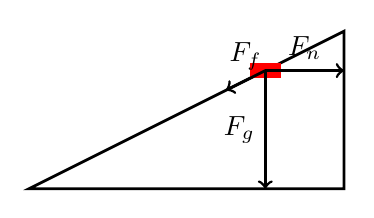
\begin{tikzpicture}
  % Draw inclined plane
  \draw[line width=1pt] (0,0) -- (4,0) -- (4,2) -- cycle;

  % Draw box
  \fill[red] (2.8,1.4) rectangle (3.2,1.6);

  % Draw and label forces
  \draw[->,line width=1pt] (3,1.5) -- (3,0) node[midway,left] {$F_g$};
  \draw[->,line width=1pt] (3,1.5) -- (4,1.5) node[midway,above] {$F_n$};
  \draw[->,line width=1pt] (3,1.5) -- (2.5,1.25) node[midway,above] {$F_f$};
\end{tikzpicture}
\end{document}